\documentclass[12pt,a4paper]{article}
\usepackage[utf8]{inputenc}
\usepackage{graphicx}   % Para insertar imágenes
\usepackage{amsmath}    % Para fórmulas matemáticas
\usepackage{hyperref}   % Para enlaces
\usepackage{listings}   % Para código
\usepackage{xcolor}

% Configuración para mostrar código Python
\lstset{
    language=Python,
    backgroundcolor=\color{white},
    basicstyle=\ttfamily\small,
    keywordstyle=\color{blue},
    commentstyle=\color{green!50!black},
    stringstyle=\color{red},
    showstringspaces=false,
    frame=single,
    breaklines=true
}

\title{INFORME PROYECTO DE FISICA}
\author{Alcazar Ureña Ariel Alexander \\ Amelunge Guzmán Leonardo Matías \\ Moya Argollo Daniela Valery \\ Ochoa Jhonatan Williams \\ Ortuño Cespedes Leandro Andre \\ Romero Aguilar Joan Matias}
\date{\today}

\usepackage{float}

\begin{document}

\maketitle


\section{INTRODUCCIÓN}
Este informe presenta el desarrollo del proyecto de Física Teórica, incluyendo la metodología, 
las fórmulas matemáticas utilizadas, la implementación en Python y los resultados obtenidos.

\subsection{¿Qué es cinemática?}
El estudio de la cinemática permite analizar y predecir el movimiento de los cuerpos en función del tiempo. 
En este proyecto se aborda un problema clásico de dos automóviles que se desplazan en la misma dirección, 
uno con velocidad constante y otro con aceleración constante. El objetivo es determinar la velocidad necesaria 
para que el automóvil A nunca rebase al automóvil B, aplicando las ecuaciones de MRU y MRUA. 
Además, se busca integrar la resolución matemática con herramientas computacionales como Python y documentar 
el proceso en LaTeX para obtener un informe académico claro y estructurado.

\section{OBJETIVOS}
\subsection{Objetivo General}
Determinar la velocidad del automóvil A que garantiza que no se acerque a menos de 10 metros del automóvil B, 
utilizando las ecuaciones de movimiento rectilíneo uniforme y uniformemente acelerado.

\subsection{Objetivos Específicos}
\begin{itemize}
    \item Plantear las ecuaciones de movimiento para ambos automóviles.
    \item Identificar el tipo de movimiento de cada automóvil (MRU y MRUA).
    \item Resolver matemáticamente el problema aplicando derivadas para encontrar la distancia mínima.
    \item Implementar el cálculo en Python para verificar los resultados.
    \item Documentar el proceso completo en LaTeX, incluyendo fórmulas, código y capturas de simulación.
\end{itemize}

\section{METODOLOGÍA}
El desarrollo del proyecto se realizó siguiendo los siguientes pasos:
\begin{enumerate}
    \item \textbf{Planteamiento del problema:} Se definieron las condiciones iniciales de los automóviles, 
    incluyendo velocidades, aceleración y distancia inicial.
    \item \textbf{Formulación matemática:} Se establecieron las ecuaciones de movimiento para cada automóvil 
    y la expresión de la distancia entre ellos.
    \item \textbf{Análisis:} Se aplicó cálculo diferencial para determinar el instante en que la distancia 
    entre los automóviles es mínima.
    \item \textbf{Resolución:} Se impuso la condición de distancia mínima de 10 metros y se resolvió para 
    obtener la velocidad del automóvil A.
    \item \textbf{Implementación computacional:} Se programó el modelo en Python para comprobar los resultados 
    y generar simulaciones.
    \item \textbf{Documentación:} Se redactó el informe en LaTeX, integrando teoría, fórmulas, código y 
    capturas de simulación.
\end{enumerate}


\section{MARCO TEÓRICO: MRU y MRUA}

En este ejemplo se combinan dos tipos de movimiento:

\subsection{Movimiento Rectilíneo Uniforme (MRU)}
Se caracteriza por una velocidad constante y trayectoria recta.  
La ecuación de posición es:


\[
x(t) = x_0 + v \cdot t
\]


En el problema, el automóvil A se mueve con velocidad constante \(v_A\), por lo tanto su movimiento es MRU.

\subsection{Movimiento Rectilíneo Uniformemente Acelerado (MRUA)}
Se caracteriza por una aceleración constante.  
Las ecuaciones de movimiento son:


\[
v(t) = v_0 + a \cdot t
\]




\[
x(t) = x_0 + v_0 \cdot t + \tfrac{1}{2} a t^2
\]


En el problema, el automóvil B parte con velocidad inicial \(v_B\) y acelera con \(a = 1 \,\text{m/s}^2\), por lo tanto su movimiento es MRUA.

\section{HERRAMIENTAS}

Las herramientas que se implemento dentro del proyecto son:
\begin{enumerate}
\item \textbf{Git:} Es un sistema de control de versiones que permite guardar y gestionar cambios en el código a lo largo del tiempo.
\item \textbf{Github:} Plataforma en línea que permite almacenar repositorios de código y colaborar en proyectos.
\item \textbf{Editor de código:} Software donde se escribe y ejecuta el programa (por ejemplo: Visual Studio Code).
\item \textbf{LateX:} Sistema utilizado para escribir fórmulas matemáticas y documentos científicos con formato profesional.
\item \textbf{Manim:} Biblioteca de Python utilizada para crear animaciones matemáticas y gráficas, ideal para visualizar el movimiento de los automóviles en este problema.
\item \textbf{Programación Orientada a Objetos (POO):} Paradigma de programación que organiza el código en objetos (por ejemplo, un objeto “Automóvil” con propiedades como velocidad y posición).
\item \textbf{Programación estructurada:} Forma de programar basada en el uso de funciones, secuencias y estructuras de control (if, loops), facilitando la organización del código.
\item \textbf{Overleaf:} Editor LaTeX basado en la nube, creado en 2011 por John Hammersley y John Lees-Miller. Redacción científica y técnica, especialmente artículos, tesis y presentaciones.
\item \textbf{Sympy:} Biblioteca de Python para matemáticas simbólicas (CAS: Computer Algebra System). Realizar cálculos algebraicos exactos, manipulación de expresiones y resolución de ecuaciones.
    
\end{enumerate}

\section{EJEMPLO DE CINEMATICA UNIDIMENCIONAL Num 13}
El problema consiste en determinar la velocidad del automóvil A para que nunca se acerque 
a menos de 10 m del automóvil B.



Las ecuaciones de movimiento son:




\[
x_B(t) = v_B \cdot t + \tfrac{1}{2} a t^2
\]




\[
x_A(t) = -100 + v_A \cdot t
\]



La distancia entre ellos:


\[
d(t) = 100 + (v_B - v_A) t + \tfrac{1}{2} a t^2
\]



El mínimo ocurre cuando:


\[
\frac{d}{dt} d(t) = (v_B - v_A) + a t = 0
\]



Evaluando en ese instante:


\[
d_{\min} = 100 - \frac{(v_A - v_B)^2}{2a}
\]



Imponiendo \(d_{\min} = 10\):


\[
v_A = v_B + \sqrt{180} \approx 32.9 \,\text{m/s}
\]

\section{FUNCIONES IMPLEMENTADAS CON SYMPY}

\begin{lstlisting}
t, vA = symbols('t vA')
\end{lstlisting}

```latex
\begin{lstlisting}
xa = vA*t
\end{lstlisting}

```latex
\begin{lstlisting}
v0b = round(v0b * (1000 / 3600),2)
print('v0b = ',v0b)
\end{lstlisting}

```latex
\begin{lstlisting}
xB = d0 + (v0b*t) + (0.5*aB*t**2)
\end{lstlisting}

```latex
\begin{lstlisting}
d = xB - xa
print('d =', xB,'-', xa)
\end{lstlisting}

```latex
\begin{lstlisting}
deriv = diff(d, t)
print('0 =',deriv)
\end{lstlisting}

```latex
\begin{lstlisting}
t_ecua = solve(deriv, t)[0]
print('t =',t_ecua)
\end{lstlisting}

```latex
\begin{lstlisting}
xB_sus = xB.subs(t, t_ecua)
xa_sus = xa.subs(t, t_ecua)
ec_2 = xB.subs(t, t_ecua) - xa.subs(t, t_ecua)
ec_2_res = simplify(ec_2)
print(dmin,'=',ec_2_res)
\end{lstlisting}

```latex
\begin{lstlisting}
res = Eq(dmin * 2, ec_2_res * 2)
print('vA**2 = ',solve(res, vA**2)[0])
\end{lstlisting}

```latex
\begin{lstlisting}
vA_sol = (solve(ec_2_res - dmin, vA))
sol_redon = [round(float(s), 2) for s in vA_sol]
print(sol_redon)
\end{lstlisting}

\subsection{Resultados de SymPy}


\[
\begin{aligned}
v_{0B} &= 19.44 \\
d &= 0.5t^{2} + 19.44t + 100 - t v_{A} \\
0 &= 1.0t - v_{A} + 19.44 \\
t &= v_{A} - 19.44 \\
10 &= 19.44v_{A} + 0.5(v_{A} - 19.44)^{2} - 277.9136 - v_{A}(v_{A} - 19.44) \\
10 &= -0.5v_{A}^{2} + 19.44v_{A} - 88.9568 \\
20 &= -1.0v_{A}^{2} + 38.88v_{A} - 177.9136 \\
v_{A}^{2} &= 38.88v_{A} - 197.9136 \\
v_{A} &= \{6.02,\ 32.86\}
\end{aligned}
\]


\section{EXPLICACIÓN Y RESULRADOS IMPLEMENTANDO PYTHON}

\subsection{Diagrama de Flujo}

En esta sección se muestra el diagrama de flujo del proyecto, implementando el proceso de las cuatro clases: \\ Main.py \\ Persecución.py \\ Resolución.py \\ Vehículo.py

\begin{figure}[H]
    \centering
    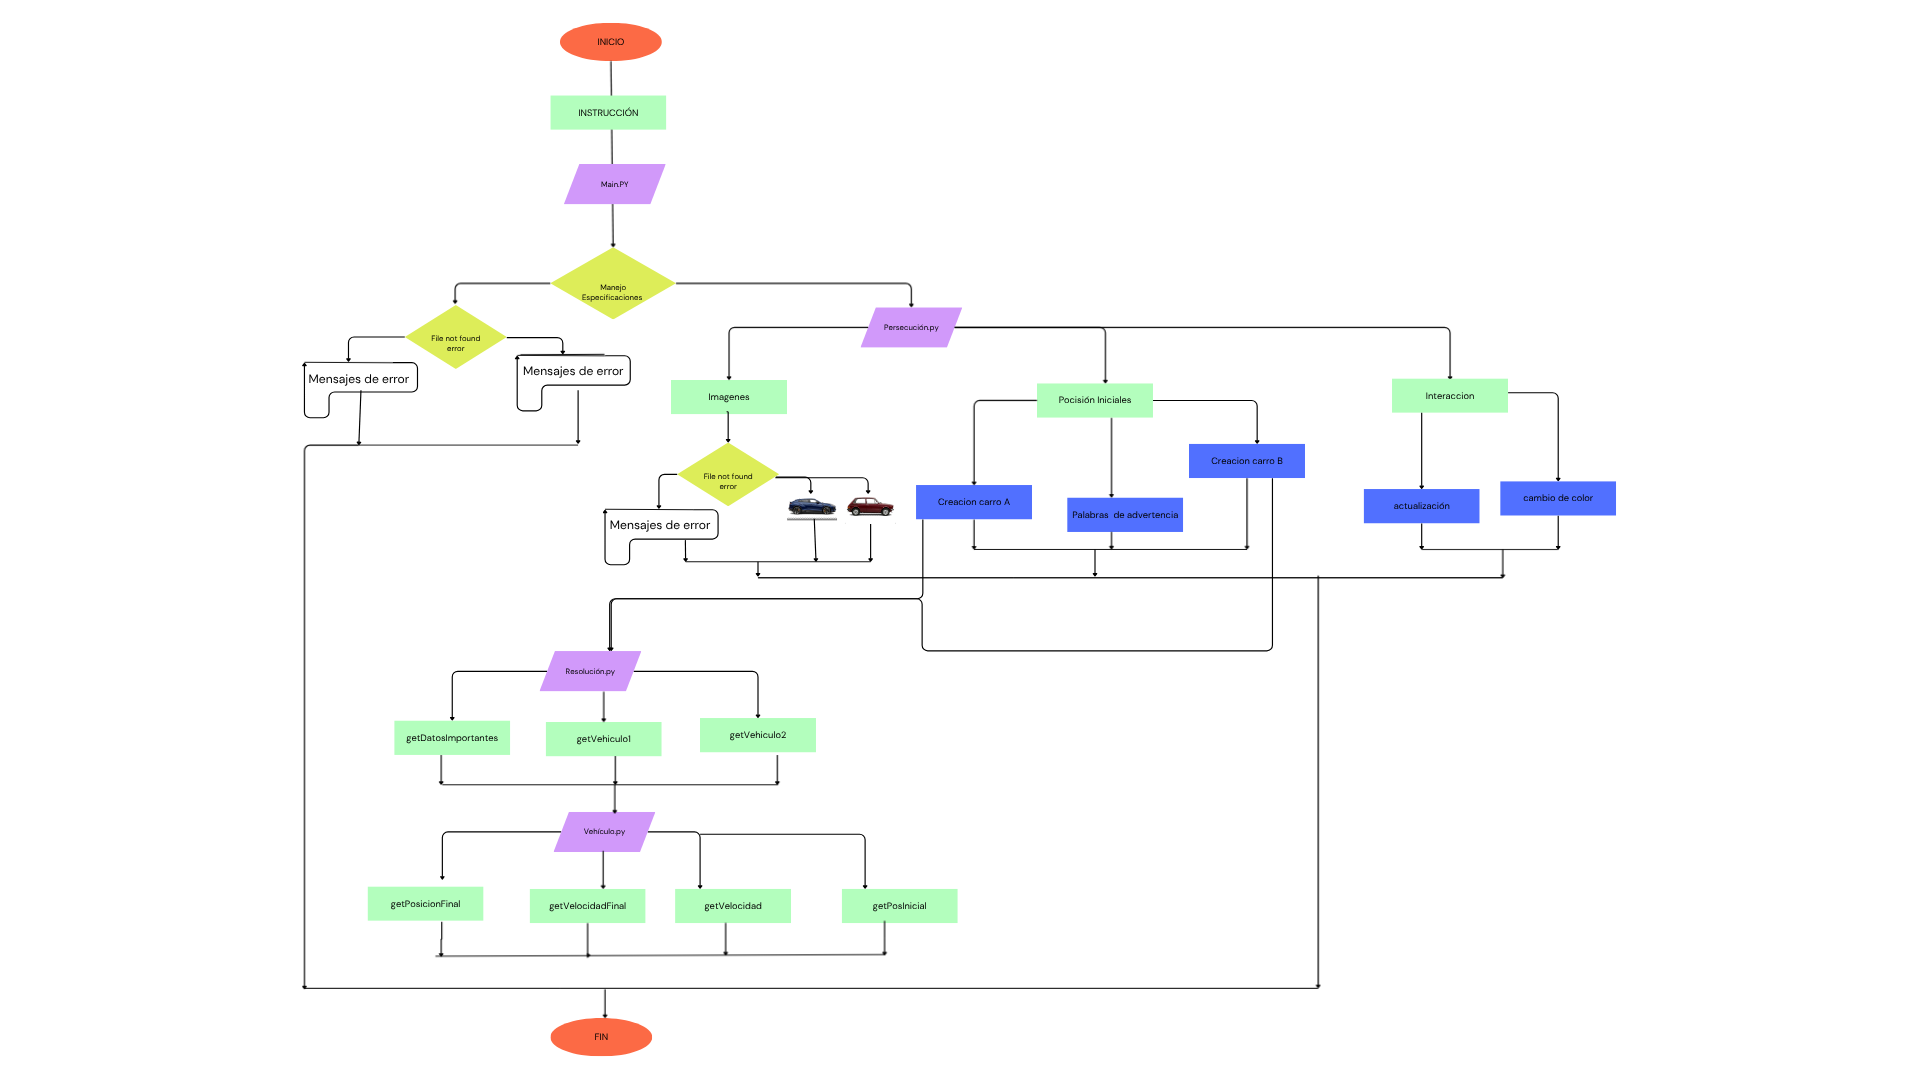
\includegraphics[width=0.7\textwidth]{frame11.png}
    \caption{Fotograma completo del diagrama de flujo.}
\end{figure}

\begin{figure}[H]
    \centering
    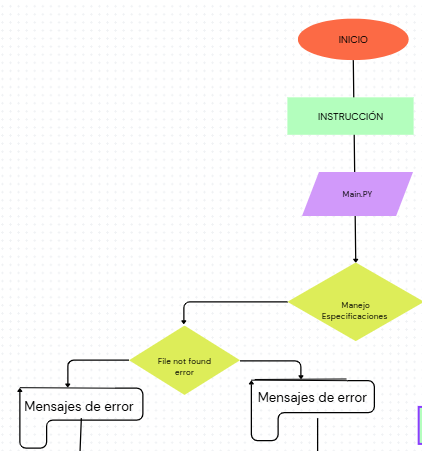
\includegraphics[width=0.7\textwidth]{frame12.png}
    \caption{Fotograma del diagrama de flujo de la clase Main.py.}
\end{figure}

\begin{figure}[H]
    \centering
    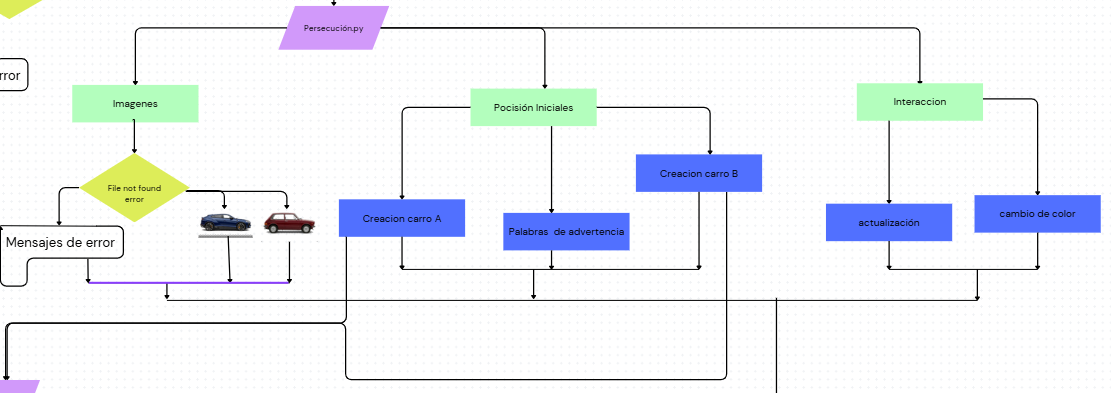
\includegraphics[width=0.7\textwidth]{frame13.png}
    \caption{Fotograma del diagrama de flujo de la clase Persecución.py.}
\end{figure}

\begin{figure}[H]
    \centering
    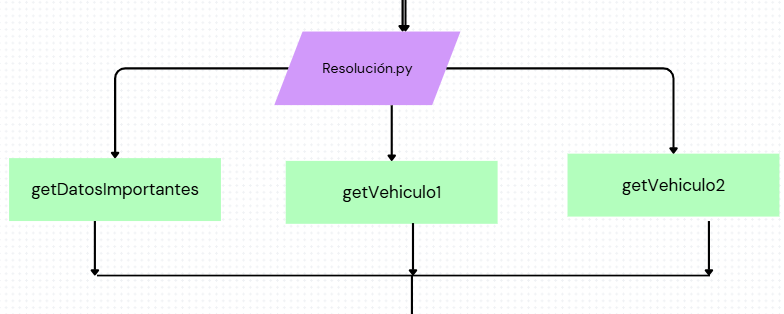
\includegraphics[width=0.7\textwidth]{frame14.png}
    \caption{Fotograma del diagrama de flujo de la clase Resolución.py.}
\end{figure}

\begin{figure}[H]
    \centering
    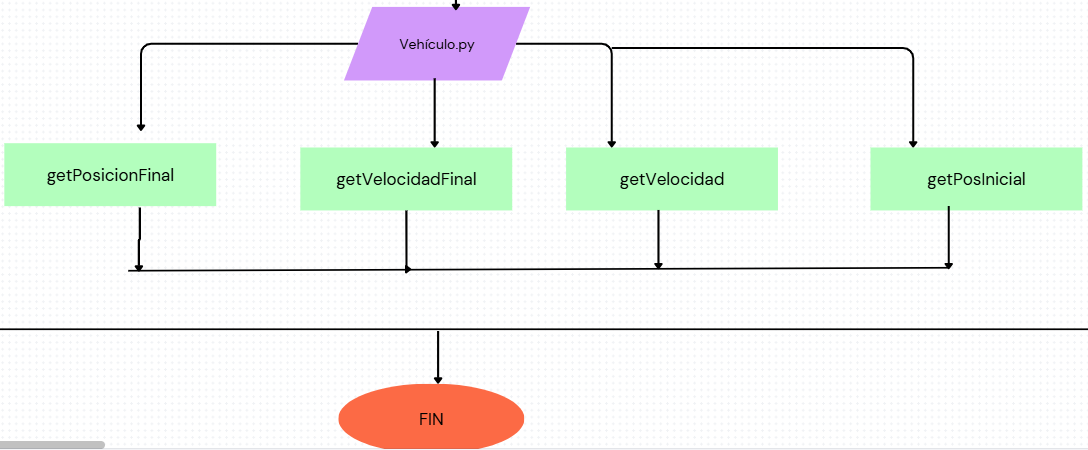
\includegraphics[width=0.7\textwidth]{frame15.png}
    \caption{Fotograma del diagrama de flujo de la clase Vehículo.py.}
\end{figure}


\subsection{Código Python}
En esta parte del proyecto entra el verdadero reto de la programación, ya que estamos creando la simulación del el ejercicio 13 de la practica de Cinematica Unidimensional a base de código usando herramientas como Manim, Math, creando la interacción entre objetos, tratando de siempre enfocarnos en tener buenas prácticas a lo largo del desarrollo como ser: Nombres Autodescriptivos, Código legible, limpio y mantenible, respetando el mismo formato de escritura PascalCase. \\ Para ello el proyecto se estructuró de la siguiente manera: \\ Clases:

\begin{enumerate}
\item \textbf{Vehículo.py :} En este Archivo se creó la clase Vehiculo para crear el comportamiento y características que tiene UN solo vehículo, teniendo el enfoque de los pilares fundamentales de la Programación Orientada a Objetos(POO), como ser encapsulamiento, abstracción, teniendo métodos que acceso a las características de cada vehículo(métodos get) para el correcto comportamiento al momento de la simulación.

\begin{figure}[H]
    \centering
    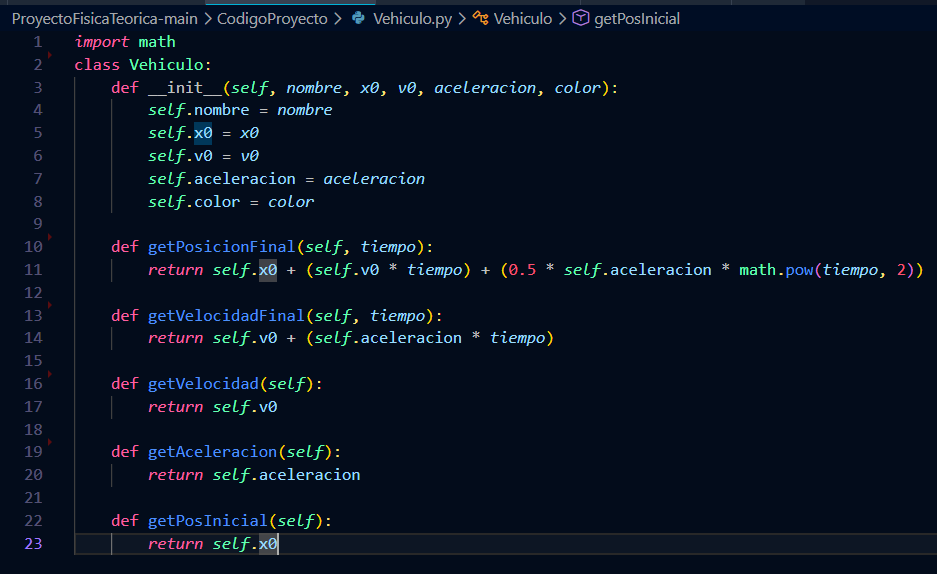
\includegraphics[width=0.7\textwidth]{frame1.png}
    \caption{Clase Vehículo del codigo.}
\end{figure}


\item \textbf{Resolución.py :} En este archivo se implementó la interacción con la clase Vehículo, una vez construidos los dos Vehículos en la clase Resolución, se creó métodos de acceso(métodos get) para que sea más sencillo  obtener datos de los Vehículos

\begin{figure}[H]
    \centering
    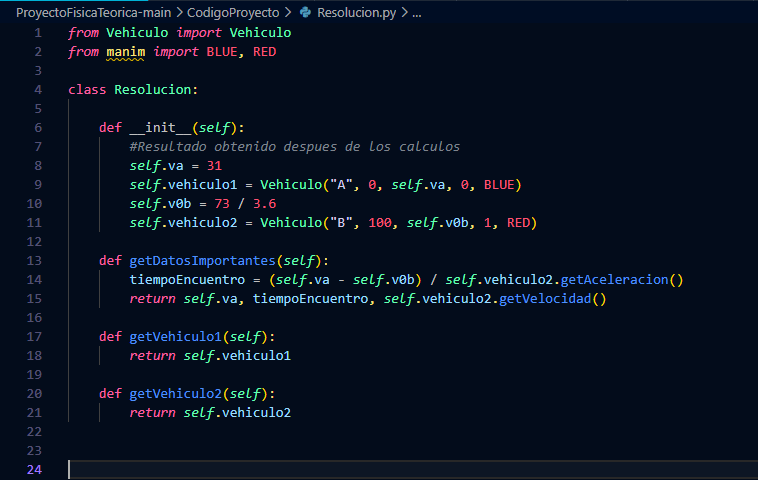
\includegraphics[width=0.7\textwidth]{frame2.png}
    \caption{Clase Resolución del código.}
\end{figure}

\item \textbf{Persecusión.py :} En este archivo se creó la “magia” de la simulación, se la dividió en 2 partes muy importantes, un método constructor y gestor de flujos que sería donde se invocan todos los métodos que se implementaron y una segunda parte donde esta desarrollados todos los métodos auxiliares necesarios para el proyecto, en este archivo se enfocó las buenas prácticas ya que es el archivo más grande del proyecto, usando todas las herramientas necesarias como ser: estructuras de control condicional, estructuras de control de excepciones, construcción de la escena usando Manim,etc.
\\ Métodos usados en todo el archivo:
\begin{itemize}
\item construct: Método constructor y gestor de flujos en el desarrollo de la simulación
\item imagenes: Método encargado de cargar las imágenes de los autos, almacenados en un archivo aparte, usando una estructura de excepciones 
\item posicionesIniciales: Método encargado de almacenar los datos iniciales de los dos vehículos, estos datos los obtiene invocando a los objetos de los vehículos desde sus métodos de acceso.
\item interraccion: Método encargado de la ”interacción” de los dos vehículos, acá es donde se actualiza los datos de los vehículos conforme se lleva a cabo la simulación, se creó una flecha dinámica que cambia su tamaño y su color una vez se van acercando, para ello lo logra teniendo sus métodos auxiliares como ser:
\item actualizacion: Método encargado de actualizar los valores de los vehículos y el color y tamaño de la flecha.
\item colorFlecha: Método donde cambia el color de la flecha una vez empieza a reducir su tamaño.
\end{itemize}


\begin{figure}[H]
    \centering
    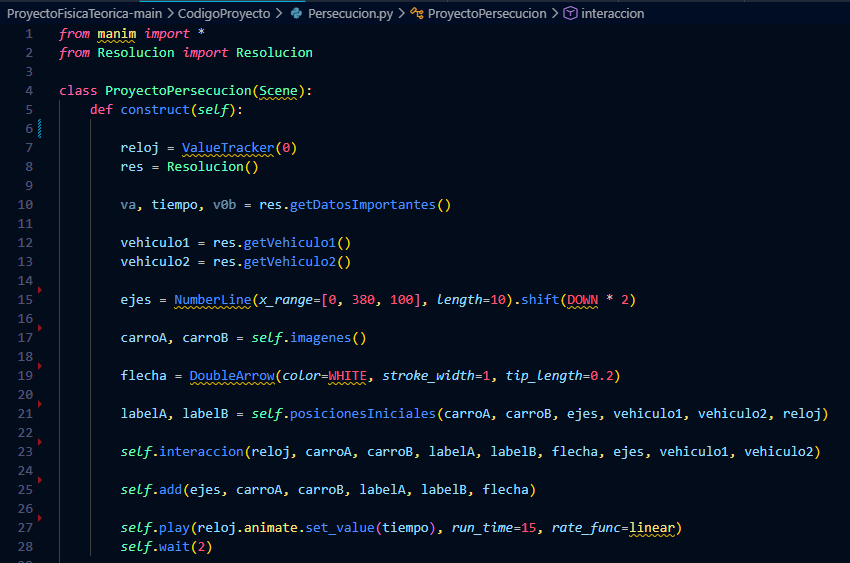
\includegraphics[width=0.7\textwidth]{frame3.png}
    \caption{Clase Persecución del código primera parte.}
\end{figure}

\begin{figure}[H]
    \centering
    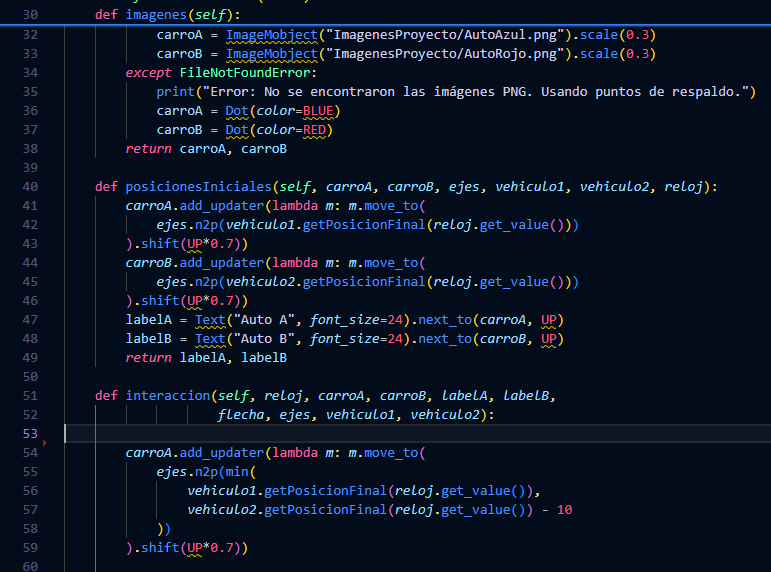
\includegraphics[width=0.7\textwidth]{frame4.png}
    \caption{Clase Persecución del código segunda parte.}
\end{figure}

\begin{figure}[H]
    \centering
    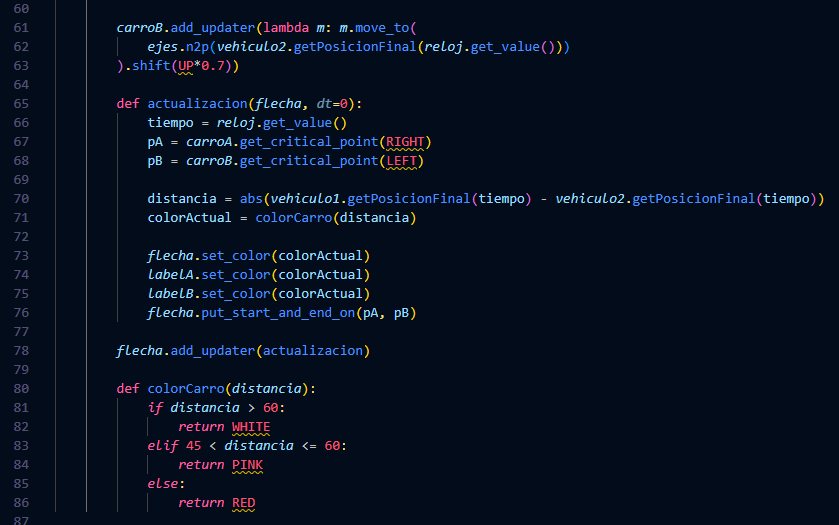
\includegraphics[width=0.7\textwidth]{frame5.png}
    \caption{Clase Persecución del código tercera parte.}
\end{figure}

\item \textbf{Main.py :} Se implementó este archivo por el motivo de tener un “Administrador” de las clases, con solo ejecutar esta clase funcione todo lo que viene siendo la simulación, para  ello se usó herramientas poderosas e importantes  como ser:
Subprocess y Sys. La implementación de estos módulos permite que el proyecto cumpla con el principio de encapsulamiento, donde el usuario final interactúa con una interfaz simple (un solo script de ejecución) mientras que la complejidad técnica del renderizado matemático queda oculta y gestionada por el Administrador del Sistema, para ello se implementó una estructura de manejo de excepciones. "La inclusión de este mecanismo de control asegura que el 'Administrador' no solo ejecute las tareas, sino que también supervise la integridad de los procesos, proporcionando un entorno de ejecución seguro y controlado para la simulación física


\begin{figure}[H]
    \centering
    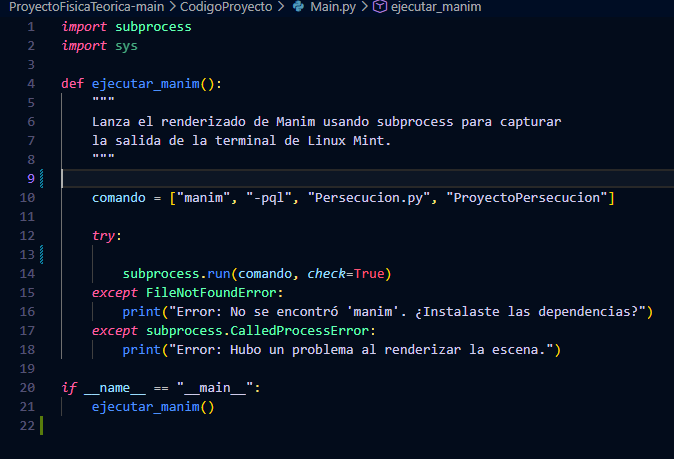
\includegraphics[width=0.7\textwidth]{frame6.png}
    \caption{Clase Principal del código}
\end{figure}

\end{enumerate}

\subsection{Simulación}

En esta sección se muestran los resultados de la simulación paso a paso, acompañados de imágenes representativas:

\begin{figure}[H]
    \centering
    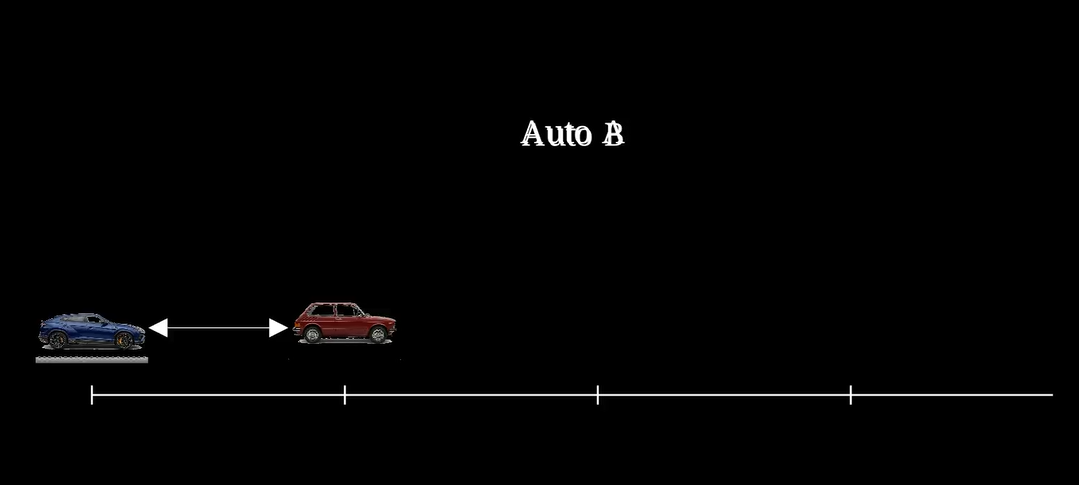
\includegraphics[width=0.7\textwidth]{frame7.png}
    \caption{Primer fotograma de la simulación.}

    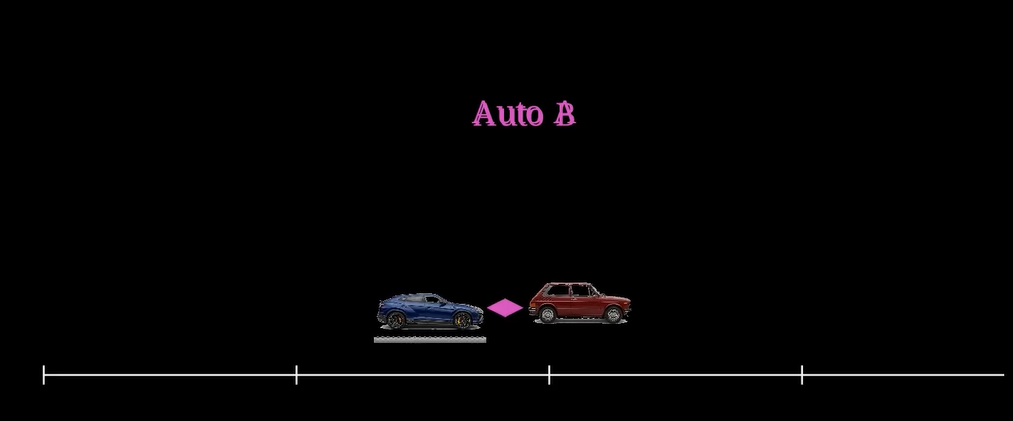
\includegraphics[width=0.7\textwidth]{frame8.png}
    \caption{Segundo fotograma de la simulación.}

    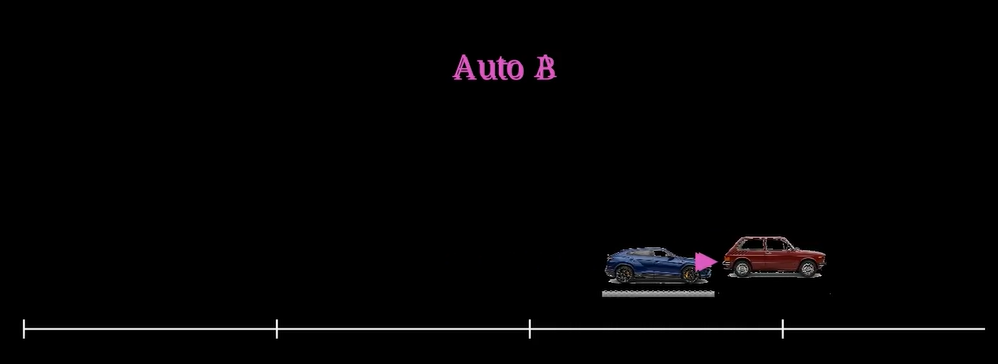
\includegraphics[width=0.7\textwidth]{frame9.png}
    \caption{Tercer fotograma de la simulación.}

    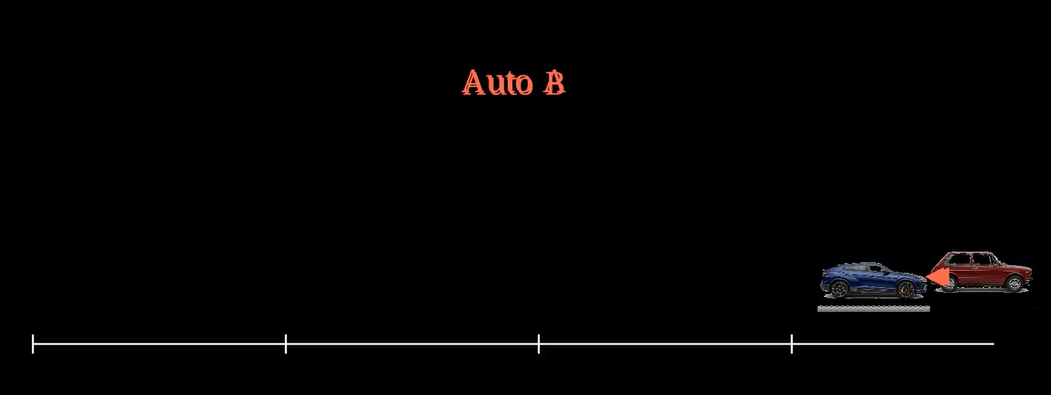
\includegraphics[width=0.7\textwidth]{frame10.png}
    \caption{Cuarto fotograma de la simulación.}
\end{figure}


\section{Conclusiones}
Se integraron las ecuaciones de cinemática en un modelo computacional con Python, 
documentado en LaTeX, obteniendo un resultado consistente con la teoría.


\begin{itemize}
    \item Se identificó correctamente el tipo de movimiento de cada automóvil: MRU para el automóvil A y MRUA para el automóvil B.
    \item Se aplicaron las ecuaciones de movimiento y el cálculo diferencial para determinar la condición de distancia mínima entre ambos vehículos.
    \item Se comprobó que la velocidad del automóvil A debe ser aproximadamente \(32.9 \,\text{m/s}\) para garantizar que nunca se acerque a menos de 10 metros del automóvil B.
    \item La implementación en Python permitió verificar los resultados teóricos y generar simulaciones que refuerzan la comprensión del problema.
    \item La documentación en LaTeX aseguró una presentación clara, estructurada y académica del proceso completo, integrando teoría, fórmulas, código y capturas de simulación.
\end{itemize}

En conclusión, el proyecto demuestra la importancia de combinar fundamentos teóricos, herramientas computacionales y una adecuada documentación científica para abordar problemas de física aplicada. Esta integración no solo facilita la resolución precisa, sino que también fortalece las competencias en programación, análisis matemático y comunicación académica.


\end{document}
